\documentclass{beamer}

% packages
\usepackage{graphicx}
  \graphicspath{{figures}}
\usepackage{minted}

% subfig support
\usepackage{caption}
\usepackage{subcaption}

% theme info
\usetheme{firedrake}

% title info
\title{\texttt{pyop3}: A (semi-)novel abstraction for automating mesh-based computations}
\author{Connor Ward}
\date{September 2022}

\begin{document}

\frame{\titlepage}

\section{State of play}

\begin{frame}
  \frametitle{PyOP2}

  \large
  \textit{PyOP2 is a framework for automating mesh-based computations.}
  \normalsize

  \begin{itemize}
    \item
      \textit{``automating"} means \textit{"using code generation"}
    \item
      \textit{``mesh-based computations"} = \textit{Next slide...}
    \item
      Integral\footnote{Pun intended.} part of the Firedrake finite element system.
    \item
      Support for iteration over extruded meshes (discussed later).
  \end{itemize}
\end{frame}

\begin{frame}
  \frametitle{``Mesh-based computations"}

  \begin{enumerate}
    \item Loop over a set of mesh entities (e.g. cells).
    \item Gather (pack) local data\footnote{e.g. ``all DoFs contained within the cell's closure"} from global data structure(s) into temporary array(s).
    \item Execute a local computation on this packed data.
    \item Scatter (unpack) the result of the local computation back into some global object.
  \end{enumerate}
\end{frame}

\begin{frame}
  \frametitle{DMPlex}

  \begin{itemize}
    \item
      PETSc's unstructured mesh topology abstraction.
    \item
      Dimension-independent.
  \end{itemize}

  \begin{figure}
    \centering
    \begin{subfigure}[b]{0.6\textwidth}
      \centering
      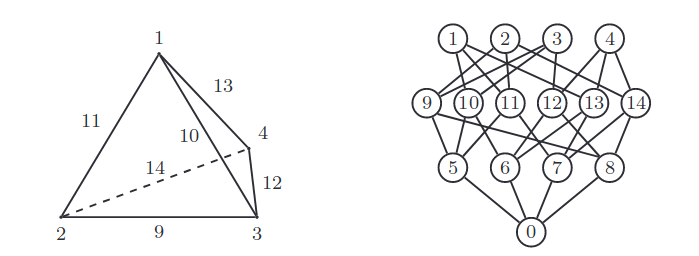
\includegraphics[width=\textwidth]{hasse}
    \end{subfigure}
    \\
    \begin{subfigure}[b]{0.3\textwidth}
      \centering
      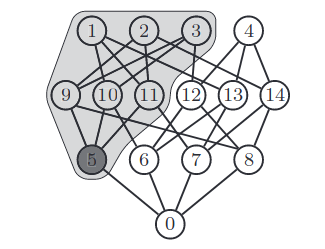
\includegraphics[width=\textwidth]{closure}
    \end{subfigure}
    \begin{subfigure}[b]{0.3\textwidth}
      \centering
      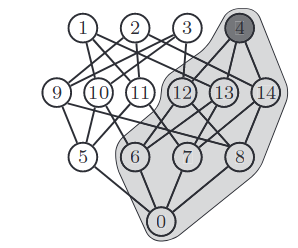
\includegraphics[width=\textwidth]{star}
    \end{subfigure}
    \caption{Source: Lange et al. (2016)}
  \end{figure}
\end{frame}

\section{What I'm doing}

\begin{frame}
  \frametitle{\texttt{pyop3}}

  \texttt{pyop3} is a total rewrite of PyOP2 that\dots

  \begin{itemize}
    \item Has improved composability (e.g. nested loops, map composition, multiple kernels)
    \item Facilitates some performance optimisations (e.g. loop tiling, loop fusion, data layout transformations)\footnote{Not yet implemented.}
    \item \textbf{Can generate fast code for a wide variety of composed meshes}
  \end{itemize}
\end{frame}

\begin{frame}[containsverbatim]
  \frametitle{pyop3 interface}

  \tiny
  \begin{minted}{python}
# cell assembly
loop(c := mesh.cells.index, kernel(dat1[closure(c)], dat2[closure(c)]))

# interior facet assembly
loop(f := mesh.interior_facets.index, [
  kernel(dat1[closure(support(f))], dat2[closure(support(f))])
])

# patches
loop(v := mesh.verts.index, [
  loop(p := star(v), kernel(dat1[closure(p)], dat2[closure(p)])),
  ...
])
  \end{minted}
\end{frame}

\begin{frame}
  \frametitle{What does ``fast code" mean?}

  \begin{itemize}
    \item
      Accessing data on unstructured meshes is slower than for structured since we need to use indirection maps (i.e. \mintinline{c}{dat[map[i]]} instead of \mintinline{c}{dat[f(i)]}).
    \item
    There are circumstances where one can have meshes with structured and unstructured bits (a.k.a. a \textit{composed} mesh).
    \item
      We want to be able to generate code that uses direct addressing for the structured parts and indirection maps for the unstructured parts.
  \end{itemize}
\end{frame}

\begin{frame}
  \frametitle{Some example meshes: extruded}

  \begin{itemize}
    \item
      Tensor product of an unstructured base mesh with a 1D interval mesh (structured).
    \item
      Iteration up columns is fast.
    \item
      Hackily supported in PyOP2.
  \end{itemize}

  \begin{figure}[b]
    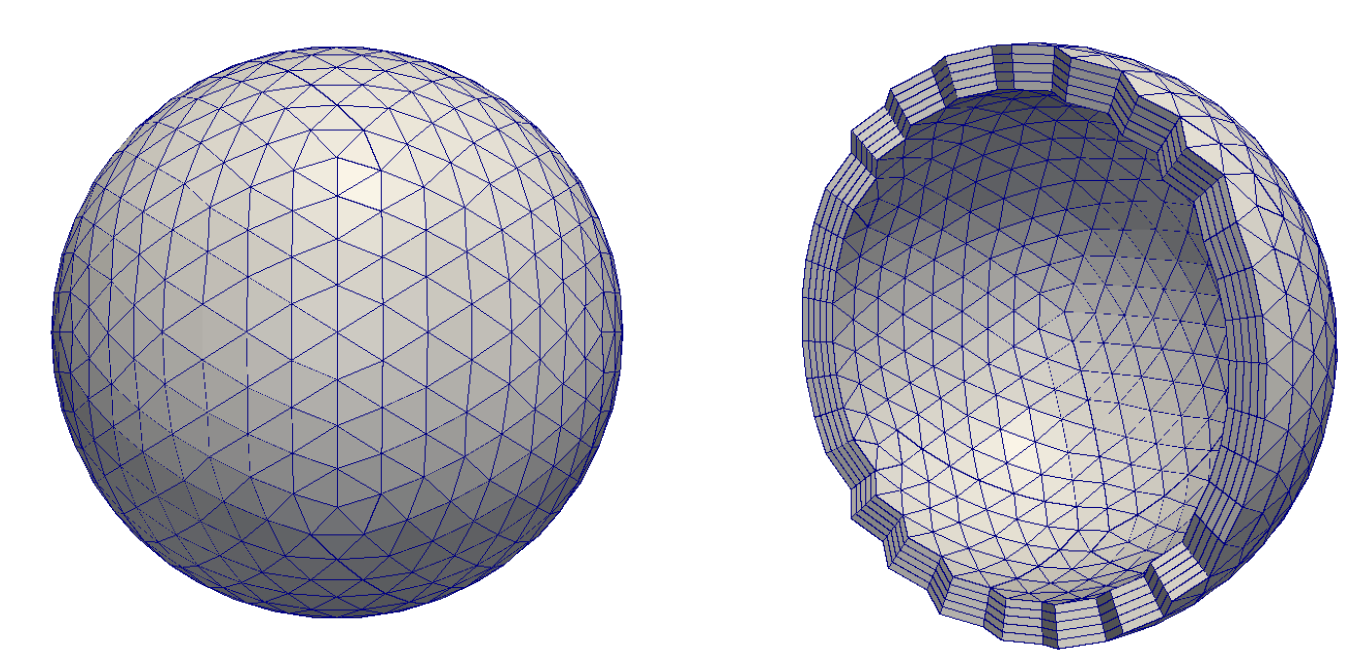
\includegraphics[width=0.7\textwidth]{extruded}
    \caption{Extruding a sphere (source: firedrakeproject.org).}
  \end{figure}
\end{frame}

\begin{frame}
  \frametitle{Some example meshes: cubed-sphere}

  \begin{itemize}
    \item
      Mesh made of 6 structured panels stuck together at the boundaries.
    \item
      Looping over the panels is fast.
  \end{itemize}

  \begin{figure}[b]
    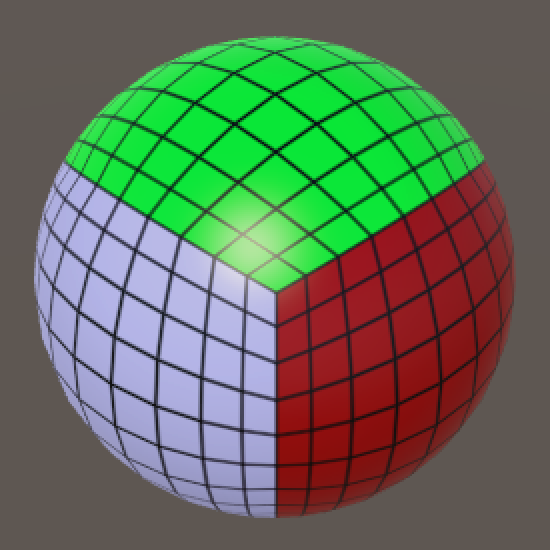
\includegraphics[width=0.45\textwidth]{cubedsphere}
    \caption{Source: catlikecoding.com}
  \end{figure}
\end{frame}

\begin{frame}
  \frametitle{Some more examples}

  \begin{itemize}
    \item Block-structured\footnote{I \textit{think} this is the correct term.} (e.g. aerofoils)
    \item Hybrid
    \item \textbf{Multigrid?}
  \end{itemize}
\end{frame}

\begin{frame}[containsverbatim]
  \frametitle{Example generated code}

  \tiny

  The pyop3 code:

  \begin{minted}{python}
loop(
  c := extruded_mesh.cells.index,
  [
    mylocalkernel(dat1[cone(c)], dat2[c])
  ]
)
  \end{minted}

  gets turned into:

  \begin{minted}{c}
double t0[16];
double t1[1];

for (int32_t i0 = 0; i0 < ncells; ++i0)  // loop over base cells
  for (int32_t i1 = 0; i1 < nlayers; ++i1)  // loop up column
  {
    for (int32_t i2 = 0; i2 < 3; ++i2)  // loop over cone of base mesh (triangles)
      for (int32_t i3 = 0; i3 < 2; ++i3)  // loop over cone of interval mesh
        for (int32_t i4 = 0; i4 < ndofs; ++i4)  // loop over DoFs
          t0[4 * i2 + 2 * i3 + i4] = dat1[
            (map0[3 * i0 + i2] * nlayers  // base cone
            + f(i1, i3)]) * ndofs  // interval cone (no map needed!)
            + i4  // DoFs
          ];
    t1[0] = 0.0;  // initialise output to zero
    mylocalkernel(&(t0[0]), &(t1[0]));  // local computation
    dat2[i0 * nlayers + i1] = t1[0];  // write to output
  \end{minted}
\end{frame}

\begin{frame}
  \frametitle{Being rigorous}

  \begin{itemize}
    \item
      We want a nice way to describe these sorts of composed meshes such that the code generation can exploit any structure.
    \item
      We, possibly erroneously, think that they might form a \textit{ring}.
      In other words, this would mean that one could \textit{add} and \textit{multiply} meshes with one another.
    \item
      For example, an extruded mesh is clearly the product of some base mesh with an interval.
  \end{itemize}
\end{frame}

\begin{frame}
  \frametitle{My questions}

  \begin{itemize}
    \item
      Is there a unified way to describe these types of mesh composition?
    \item
      How do we propagate structural information such that I can generate code to exploit it?
    \item
      Does any of the code I write belong in PETSc instead of pyop3?
  \end{itemize}
\end{frame}

\end{document}
